\documentclass[aspectratio=169]{beamer}
\usepackage[utf8]{inputenc}
\usepackage[T5]{fontenc}
\usepackage[vietnamese]{babel}
\usepackage{graphicx}
\usepackage{hyperref}
\usepackage{lmodern}

% Theme
\usetheme{Madrid}
\usecolortheme{whale}

% Metadata
\title[Các thuật toán Học máy]{Ứng dụng AI trong Nông nghiệp}
\subtitle{Chương 9: Các thuật toán Học máy}
\author{Giảng viên}
\institute{Đại học Đông Á}
\date{\today}

\begin{document}

\begin{frame}
    \titlepage
\end{frame}

\begin{frame}{Nội dung chính}
    \tableofcontents
\end{frame}

\section{Giới thiệu chung}
\begin{frame}{Thành phần chính của Học máy}
    Để mô hình học máy hoạt động và đưa ra kết quả chính xác, cần 3 thành phần chính:
    \begin{itemize}
        \item \textbf{Dữ liệu (Data):} Nguồn thông tin đầu vào (âm thanh, hình ảnh, thông số môi trường,...). Cần có bộ dữ liệu với các ví dụ đã biết nhãn (học có giám sát).
        \item \textbf{Mô hình (Model):} Cấu trúc toán học đại diện cho dữ liệu, được sử dụng để dự đoán.
        \item \textbf{Thuật toán (Algorithm):} Phương pháp để huấn luyện mô hình từ dữ liệu, giúp mô hình tìm ra quy luật hoặc mối quan hệ giữa các biến.
    \end{itemize}
\end{frame}

\section{Hồi quy tuyến tính (Linear Regression)}
\begin{frame}{1. Hồi quy tuyến tính (Linear Regression)}
    \begin{itemize}
        \item \textbf{Khái niệm:} Là thuật toán phân tích mối quan hệ giữa một (hoặc nhiều) biến độc lập (X) và một biến phụ thuộc liên tục (y).
        \item \textbf{Mục tiêu:} Tìm ra một đường thẳng (hoặc siêu phẳng) khớp nhất với dữ liệu, giúp dự đoán giá trị y từ X.
        \item \textbf{Phân loại:}
        \begin{itemize}
            \item Hồi quy tuyến tính đơn giản: 1 biến X. (Ví dụ: Dự đoán năng suất lúa dựa trên lượng phân bón).
            \item Hồi quy tuyến tính đa biến: Nhiều biến X. (Ví dụ: Năng suất lúa dựa trên lượng phân, nước, nhiệt độ).
        \end{itemize}
    \end{itemize}
\end{frame}

\begin{frame}{Minh họa Hồi quy tuyến tính}
    \begin{columns}
        \begin{column}{0.4\textwidth}
            \begin{itemize}
                \item Đường hồi quy (màu xanh) là đường thẳng đi sát nhất với các điểm dữ liệu.
                \item Sai số (chiều dọc từ điểm đến đường) được giảm thiểu tối đa (phương pháp bình phương tối thiểu - OLS).
                \item Ưu điểm: Đơn giản, dễ hiểu, tính toán nhanh.
            \end{itemize}
        \end{column}
        \begin{column}{0.6\textwidth}
            \begin{center}
                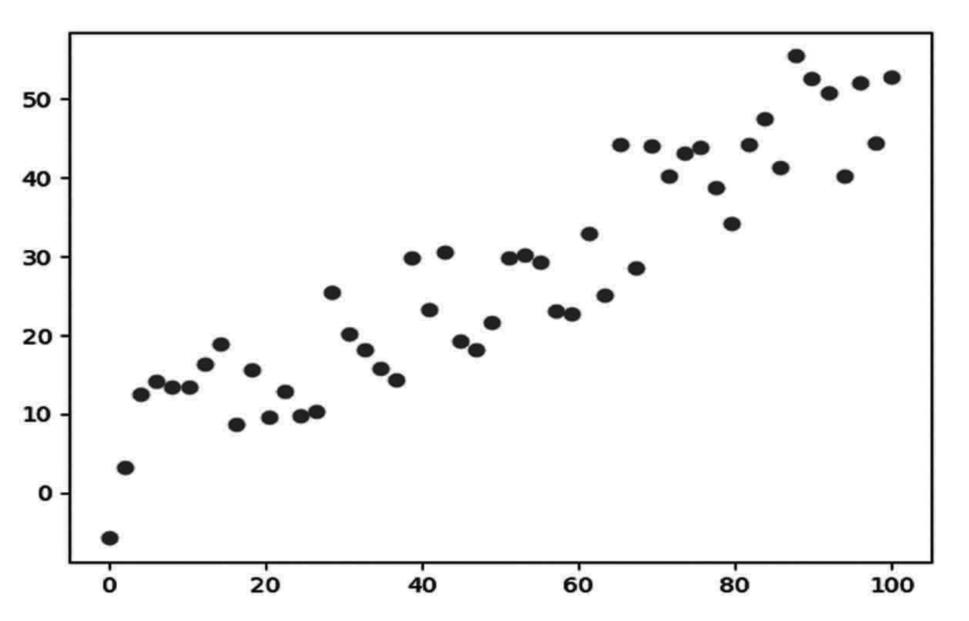
\includegraphics[width=0.9\textwidth]{chap9_img_2_0.png}
                
                \vspace{0.2cm}
                \textit{Hình 9.1: Đường Hồi quy tuyến tính}
            \end{center}
        \end{column}
    \end{columns}
\end{frame}

\section{Hồi quy Logistic}
\begin{frame}{2. Hồi quy Logistic (Logistic Regression)}
    \begin{itemize}
        \item \textbf{Khái niệm:} Dù có tên là "hồi quy", đây lại là thuật toán \textbf{phân loại}. Dùng để dự đoán xác suất xảy ra của một sự kiện.
        \item Đầu ra là giá trị xác suất từ 0 đến 1. Dựa vào một ngưỡng (thường là 0.5) để phân loại thành 2 lớp (Ví dụ: Cây mắc bệnh (1) hoặc không (0)).
        \item \textbf{Hàm Sigmoid (Logistic Function):} Đường cong chữ S giúp chuyển đổi bất kỳ giá trị thực nào về khoảng [0, 1].
    \end{itemize}
\end{frame}

\begin{frame}{Minh họa Hàm Sigmoid}
    \begin{columns}
        \begin{column}{0.4\textwidth}
            \begin{itemize}
                \item \textbf{Công thức:} $f(x) = \frac{1}{1 + e^{-x}}$
                \item Đầu ra luôn bị giới hạn từ 0 đến 1.
                \item Rất phổ biến cho bài toán phân loại nhị phân (Binary Classification) hoặc mở rộng cho đa lớp (Multi-class).
            \end{itemize}
        \end{column}
        \begin{column}{0.6\textwidth}
            \begin{center}
                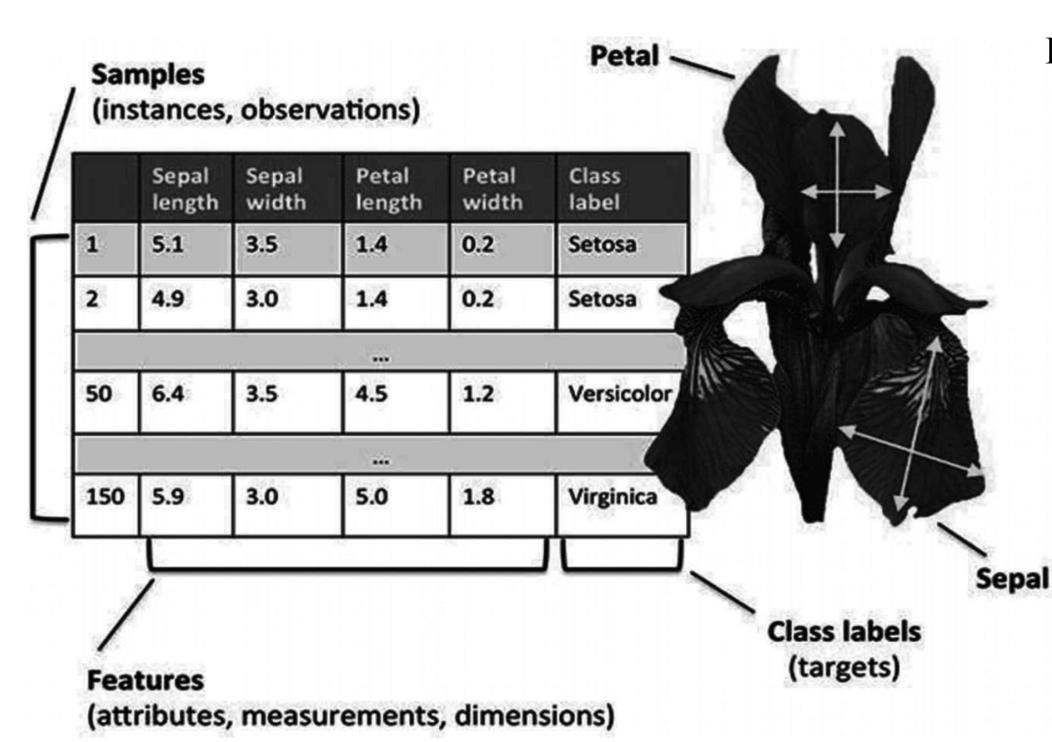
\includegraphics[width=0.9\textwidth]{chap9_img_8_0.png}
                
                \vspace{0.2cm}
                \textit{Hình 9.4: Hàm Sigmoid trong Hồi quy Logistic}
            \end{center}
        \end{column}
    \end{columns}
\end{frame}

\section{Cây quyết định (Decision Tree)}
\begin{frame}{3. Cây quyết định (Decision Tree)}
    \begin{itemize}
        \item \textbf{Khái niệm:} Thuật toán phân loại và hồi quy dưới dạng cấu trúc cây.
        \item \textbf{Cấu trúc:}
        \begin{itemize}
            \item \textbf{Nút gốc (Root Node):} Đặc trưng quan trọng nhất để bắt đầu phân chia.
            \item \textbf{Nút quyết định (Decision Node):} Các nhánh điều kiện tiếp theo.
            \item \textbf{Nút lá (Leaf/Terminal Node):} Kết quả cuối cùng (nhãn phân loại).
        \end{itemize}
        \item Việc chia nhánh dựa trên các độ đo như Entropy (độ tinh khiết) và Information Gain.
    \end{itemize}
\end{frame}

\begin{frame}{Minh họa Cây quyết định}
    \begin{columns}
        \begin{column}{0.4\textwidth}
            \begin{itemize}
                \item Mỗi nút là một câu hỏi (Ví dụ: Độ ẩm $> 60\%$?).
                \item Nếu Yes đi một nhánh, No đi nhánh còn lại.
                \item Rất dễ giải thích cho người không có chuyên môn.
            \end{itemize}
        \end{column}
        \begin{column}{0.6\textwidth}
            \begin{center}
                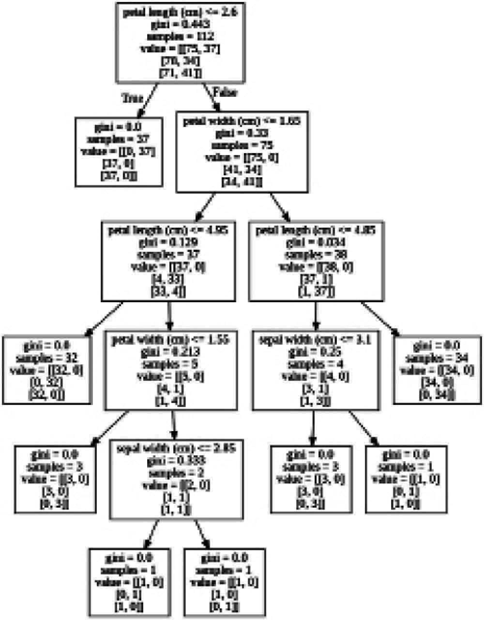
\includegraphics[height=0.65\textheight,keepaspectratio]{chap9_img_15_0.png}
                
                \vspace{0.2cm}
                \textit{Hình 9.8: Cấu trúc Cây quyết định}
            \end{center}
        \end{column}
    \end{columns}
\end{frame}

\section{Naïve Bayes}
\begin{frame}{4. Naïve Bayes}
    \begin{itemize}
        \item \textbf{Khái niệm:} Thuật toán phân loại xác suất dựa trên \textbf{Định lý Bayes}, với giả định mạnh (naïve) rằng các đặc trưng hoàn toàn độc lập với nhau.
        \item \textbf{Công thức Bayes:} $P(A|B) = \frac{P(B|A)P(A)}{P(B)}$
        \item \textbf{Ưu điểm:} 
        \begin{itemize}
            \item Tính toán cực kỳ nhanh chóng.
            \item Hiệu quả với tập dữ liệu nhỏ và đặc biệt tốt cho phân loại văn bản (như lọc email rác).
        \end{itemize}
        \item \textbf{Nhược điểm:} Giả định các đặc trưng độc lập hiếm khi đúng hoàn toàn trong thực tế.
    \end{itemize}
\end{frame}

\section{Phân cụm K-Means}
\begin{frame}{5. Phân cụm K-Means (K-Means Clustering)}
    \begin{itemize}
        \item \textbf{Khái niệm:} Thuật toán \textbf{học không giám sát} dùng để gom cụm dữ liệu chưa có nhãn.
        \item \textbf{Mục tiêu:} Phân chia dữ liệu thành $K$ cụm sao cho các điểm trong cùng 1 cụm giống nhau nhất, và các điểm giữa các cụm khác nhau nhất.
        \item \textbf{Cơ chế:} 
        \begin{itemize}
            \item Chọn $K$ tâm cụm (centroids) ngẫu nhiên.
            \item Gán mỗi điểm dữ liệu vào tâm cụm gần nhất.
            \item Cập nhật lại vị trí tâm cụm và lặp lại cho đến khi ổn định.
        \end{itemize}
    \end{itemize}
\end{frame}

\begin{frame}{Minh họa K-Means Clustering (Dữ liệu ban đầu)}
    \begin{columns}
        \begin{column}{0.4\textwidth}
            \begin{itemize}
                \item Hình bên cho thấy tập dữ liệu ban đầu gồm các điểm phân tán.
                \item Bằng mắt thường, ta có thể mường tượng được 3 cụm riêng biệt (A, B, C).
                \item Mục tiêu của thuật toán K-Means là tự động tìm ra các tâm cụm và gán nhãn cho các điểm này mà không cần dữ liệu mẫu.
            \end{itemize}
        \end{column}
        \begin{column}{0.6\textwidth}
            \begin{center}
                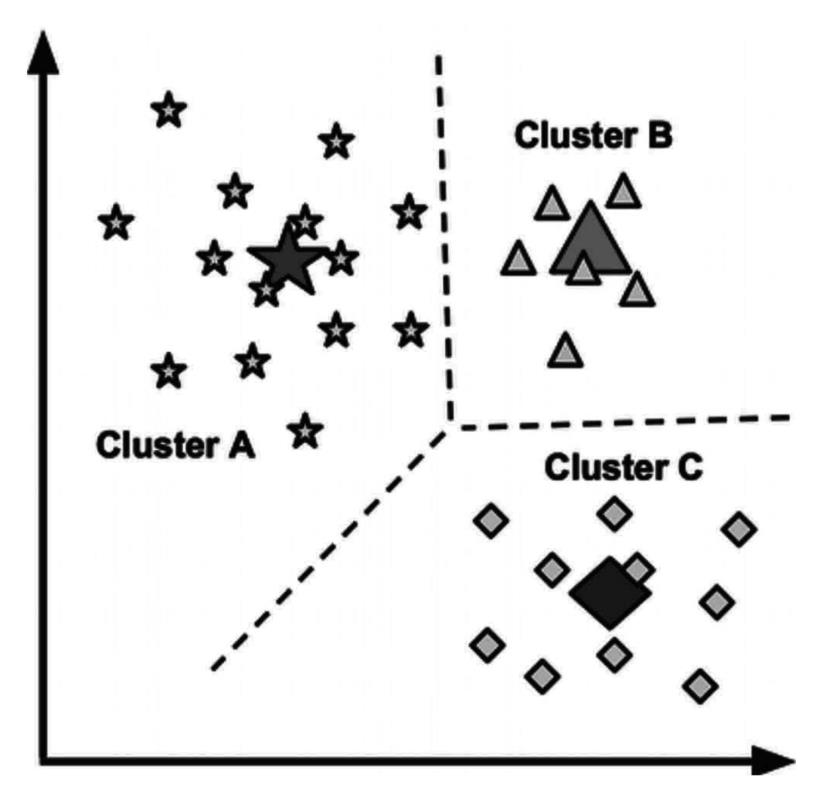
\includegraphics[width=0.9\textwidth,height=0.7\textheight,keepaspectratio]{chap9_img_30_0.png}
                
                \vspace{0.2cm}
                \textit{Hình 9.12: Dữ liệu chưa phân cụm}
            \end{center}
        \end{column}
    \end{columns}
\end{frame}

\begin{frame}{Minh họa K-Means Clustering (Kết quả phân cụm)}
    \begin{columns}
        \begin{column}{0.4\textwidth}
            \begin{itemize}
                \item Hình bên so sánh giữa cụm thực tế (Actual) và kết quả dự đoán của K-Means (Predicted).
                \item Thuật toán đã thành công trong việc gom nhóm các điểm thành các cụm có tính chất tương đồng (cùng màu).
                \item Ứng dụng phổ biến trong phân nhóm khách hàng, phân vùng đất canh tác.
            \end{itemize}
        \end{column}
        \begin{column}{0.6\textwidth}
            \begin{center}
                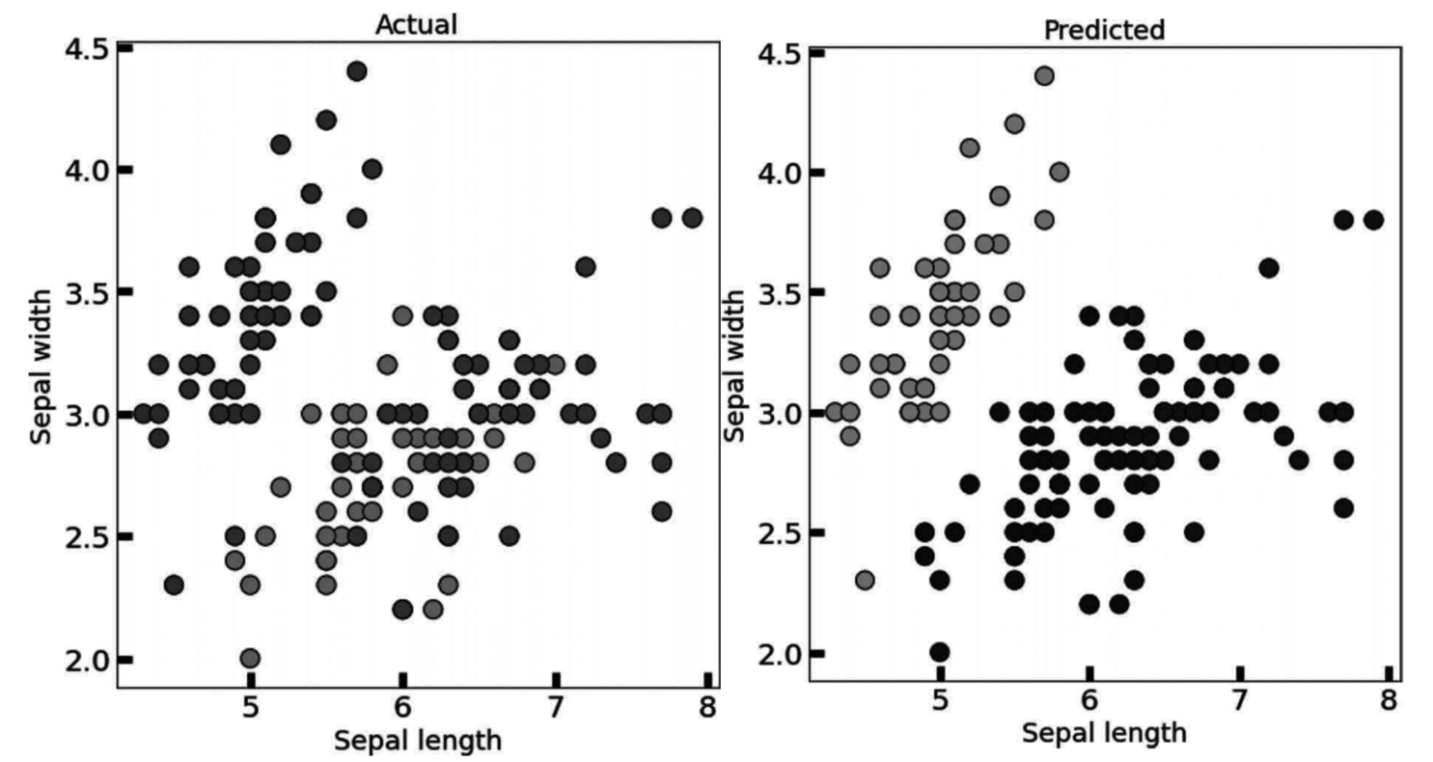
\includegraphics[width=0.9\textwidth,height=0.7\textheight,keepaspectratio]{chap9_img_32_0.png}
                
                \vspace{0.2cm}
                \textit{Hình 9.14: Kết quả phân cụm (Actual vs Predicted)}
            \end{center}
        \end{column}
    \end{columns}
\end{frame}

\section{Random Forest}
\begin{frame}{6. Rừng ngẫu nhiên (Random Forest)}
    \begin{itemize}
        \item \textbf{Khái niệm:} Thuật toán Ensemble Learning (Học tập hợp), sử dụng nhiều Cây quyết định kết hợp lại.
        \item \textbf{Cơ chế:} 
        \begin{itemize}
            \item Tạo ra nhiều cây quyết định với các tập dữ liệu con ngẫu nhiên.
            \item Khi dự đoán, mô hình tổng hợp kết quả (bỏ phiếu đa số cho phân loại, lấy trung bình cho hồi quy).
        \end{itemize}
        \item \textbf{Ưu điểm:} Tránh được hiện tượng quá khớp (overfitting) của Cây quyết định đơn lẻ, độ chính xác rất cao.
        \item \textbf{Nhược điểm:} Tính toán nặng hơn và khó giải thích trực quan hơn 1 cây đơn lẻ.
    \end{itemize}
\end{frame}

\section{Kết luận}
\begin{frame}{Tóm tắt}
    \begin{itemize}
        \item \textbf{Học có giám sát:} Linear Regression (dự báo giá trị), Logistic Regression, Decision Tree, Naïve Bayes, Random Forest (phân loại/dự báo khi có nhãn).
        \item \textbf{Học không giám sát:} K-Means (tìm cụm ẩn khi chưa có nhãn).
        \item Việc chọn thuật toán phụ thuộc vào: 
        \begin{itemize}
            \item Loại bài toán (Phân loại, Hồi quy hay Gom cụm).
            \item Số lượng và tính chất dữ liệu (Có nhãn hay không).
            \item Yêu cầu về độ chính xác vs độ dễ giải thích.
        \end{itemize}
    \end{itemize}
\end{frame}

\begin{frame}
    \begin{center}
        \Huge \textbf{Q \& A}
    \end{center}
\end{frame}

\end{document}
